%%%%%%%%%%%%%%%%%%%% author.tex %%%%%%%%%%%%%%%%%%%%%%%%%%%%%%%%%%%
%
% sample root file for your "contribution" to a contributed volume
%
% Use this file as a template for your own input.
%
%%%%%%%%%%%%%%%% Springer %%%%%%%%%%%%%%%%%%%%%%%%%%%%%%%%%%


% RECOMMENDED %%%%%%%%%%%%%%%%%%%%%%%%%%%%%%%%%%%%%%%%%%%%%%%%%%%
\documentclass[graybox]{svmult}

% choose options for [] as required from the list
% in the Reference Guide

\usepackage{mathptmx}       % selects Times Roman as basic font
\usepackage{helvet}         % selects Helvetica as sans-serif font
\usepackage{courier}        % selects Courier as typewriter font
%\usepackage{type1cm}        % activate if the above 3 fonts are
                            % not available on your system
%
\usepackage{makeidx}         % allows index generation
\usepackage{graphicx}        % standard LaTeX graphics tool
                             % when including figure files
\usepackage{multicol}        % used for the two-column index
\usepackage[bottom]{footmisc}% places footnotes at page bottom
\usepackage{amsmath,amsfonts}

% see the list of further useful packages
% in the Reference Guide

\makeindex             % used for the subject index
                       % please use the style svind.ist with
                       % your makeindex program

%%%%%%%%%%%%%%%%%%%%%%%%%%%%%%%%%%%%%%%%%%%%%%%%%%%%%%%%%%%%%%%%%%%%%%%%%%%%%%%%%%%%%%%%%

\begin{document}

\title*{The Hubness Phenomenon in High Dimensional Spaces}
% Use \titlerunning{Short Title} for an abbreviated version of
% your contribution title if the original one is too long
\author{Name of First Author and Name of Second Author}
% Use \authorrunning{Short Title} for an abbreviated version of
% your contribution title if the original one is too long
\institute{Name of First Author \at Name, Address of Institute, \email{name@email.address}
\and Name of Second Author \at Name, Address of Institute \email{name@email.address}}
%
% Use the package "url.sty" to avoid
% problems with special characters
% used in your e-mail or web address
%
\maketitle

\abstract*{Each chapter should be preceded by an abstract (10--15 lines long) that summarizes the content. The abstract will appear \textit{online} at \url{www.SpringerLink.com} and be available with unrestricted access. This allows unregistered users to read the abstract as a teaser for the complete chapter. As a general rule the abstracts will not appear in the printed version of your book unless it is the style of your particular book or that of the series to which your book belongs.
Please use the 'starred' version of the new Springer \texttt{abstract} command for typesetting the text of the online abstracts (cf. source file of this chapter template \texttt{abstract}) and include them with the source files of your manuscript. Use the plain \texttt{abstract} command if the abstract is also to appear in the printed version of the book.}

\abstract{Each chapter should be preceded by an abstract (10--15 lines long) that summarizes the content. The abstract will appear \textit{online} at \url{www.SpringerLink.com} and be available with unrestricted access. This allows unregistered users to read the abstract as a teaser for the complete chapter. As a general rule the abstracts will not appear in the printed version of your book unless it is the style of your particular book or that of the series to which your book belongs. \newline\indent
Please use the 'starred' version of the new Springer \texttt{abstract} command for typesetting the text of the online abstracts (cf. source file of this chapter template \texttt{abstract}) and include them with the source files of your manuscript. Use the plain \texttt{abstract} command if the abstract is also to appear in the printed version of the book.}

\section{Introduction}
\label{sec:1}
[Describe the phenomenon, recent observations, and open questions we are investigating here]



\section{Background and Related Work}
\label{sec:2}
% Always give a unique label
% and use \ref{<label>} for cross-references
% and \cite{<label>} for bibliographic references
% use \sectionmark{}
% to alter or adjust the section heading in the running head



\section{Intrinsic Dimensionality via Hubness}
\label{sec:3}

\subsection{Skewness vs. Feature Ranking - What is the Right Way to Rank Features? }
\label{subsec:3.1}
[Local Skewness plots, etc.]

\subsection{Supervised vs. Unsupervised Methods }
\label{subsec:3.2}
[Compare methods for feature relevance, cluster properties in original and subspace, etc.]


\section{Hubs, Density, and Clustering}
\label{sec:4}

To investigate the relationship between density, hubness scores, and clustering, data sets of 30, 60, and 100 relevant dimensions were created. For each of these dimensions, two types of data sets were generated: (1) two Gaussian spheres separated by 10 units in the first coordinate and (2) two uniform cubes separated by one unit along its first dimension. In order to emulate varying densities, one cluster was designed to contain 1000 points and the second varied in size (2000, 3000, 4000, and 5000). There was a resulting total of 24 data sets given the different dimensions, distribution of points, and varying densities. An additional non-convex data cloud in 60 dimensions composed of two close by clusters with similar density was created to measure clustering potential. For the rest of the chapter, the Gaussian data sets will be denoted as $G_{d,N}$, the uniform ones as $U_{d,N}$, where $d$ is the dimension and $N$ is the number of points, and the non-convex data cloud as $S_{60,6000}$. In general, any $d$-dimensional data of $N$ points will be denoted as $X_{d,N}$.


\subsection{Hubness and Data Density}
\label{density}

The first question to be addressed is whether hubness scores and density are the same measure. Suppose that there is a low density area, high density area, a low hubness score area and a high hubness score area, as shown in Fig. \ref{fig:DensHubInt}. Intuition dictates that if density and hubness score were correlated, all the points will lie within the first (high density and high hubness scores) and third (low density and low hubness scores) quadrants. However, if the points are all over the four quadrants, then it might imply a more complicated relationship between density and hubness scores. 

\begin{figure}
\centering
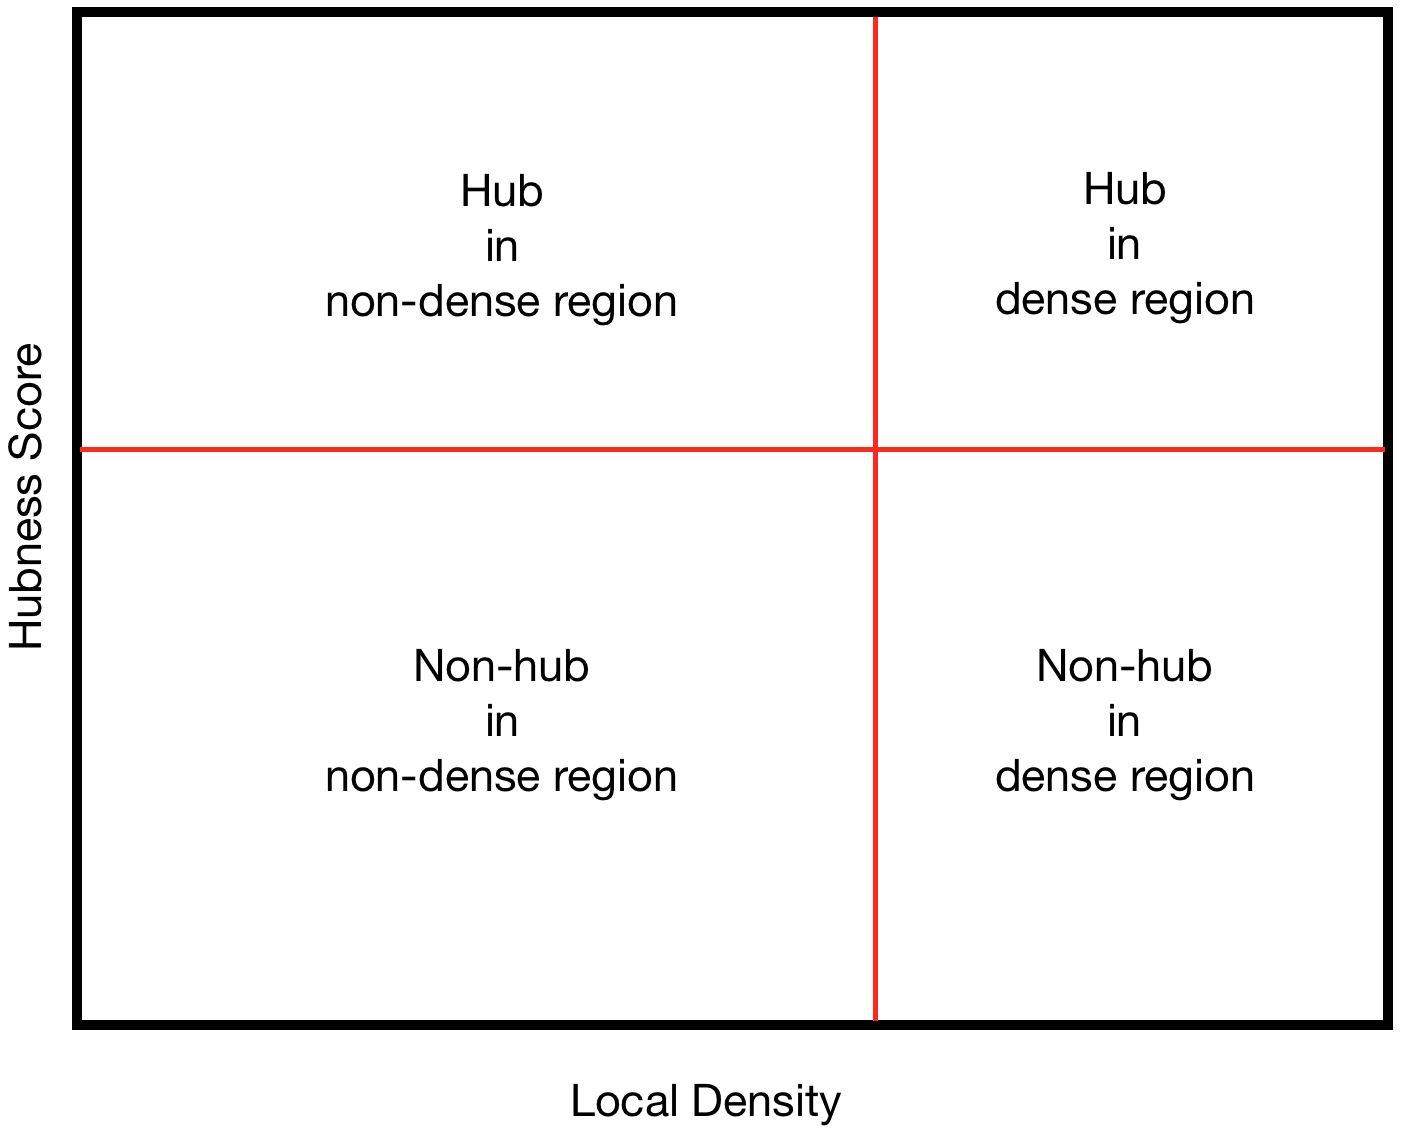
\includegraphics[width=2in,height=2in]{../fig/DensHub-Intuition.png}
\caption{An illustration of the four quadrants, which are formed by density and hubness scores thresholds, that will be seen in the following experiments where density will be plotted against hubness scores.}\label{fig:DensHubInt}
\end{figure}

To estimate density, we used the Kernel Density Estimator described in HERE with number of nearest neighbors being 100 and the bandwidth nearest neighbors being 16. The KDE is known to be an accurate consistent estimator. To determine what is ``high density'' a threshold value of two standard deviations above the mean was calculated. Also, the hubness scores $N_k$ were calculated for all the data sets with $k=5,10,$ and $50$. Taking into account the different types of data, densities, dimensions and $k$'s, there were 72 total plots.

The first set of experiments used a global threshold for the density, i.e. the mean and standard deviation were calculated for the density of all the points regardless of class membership. Some representative results are shown in Figure  \ref{GlobDensHubs}. In these figures, global thresholds for density and hubness scores were plotted in black. The blue and red represent the class membership of each point, which is known from how the data was created. 

\begin{figure}
\centering
    \begin{tabular}{cccc}
        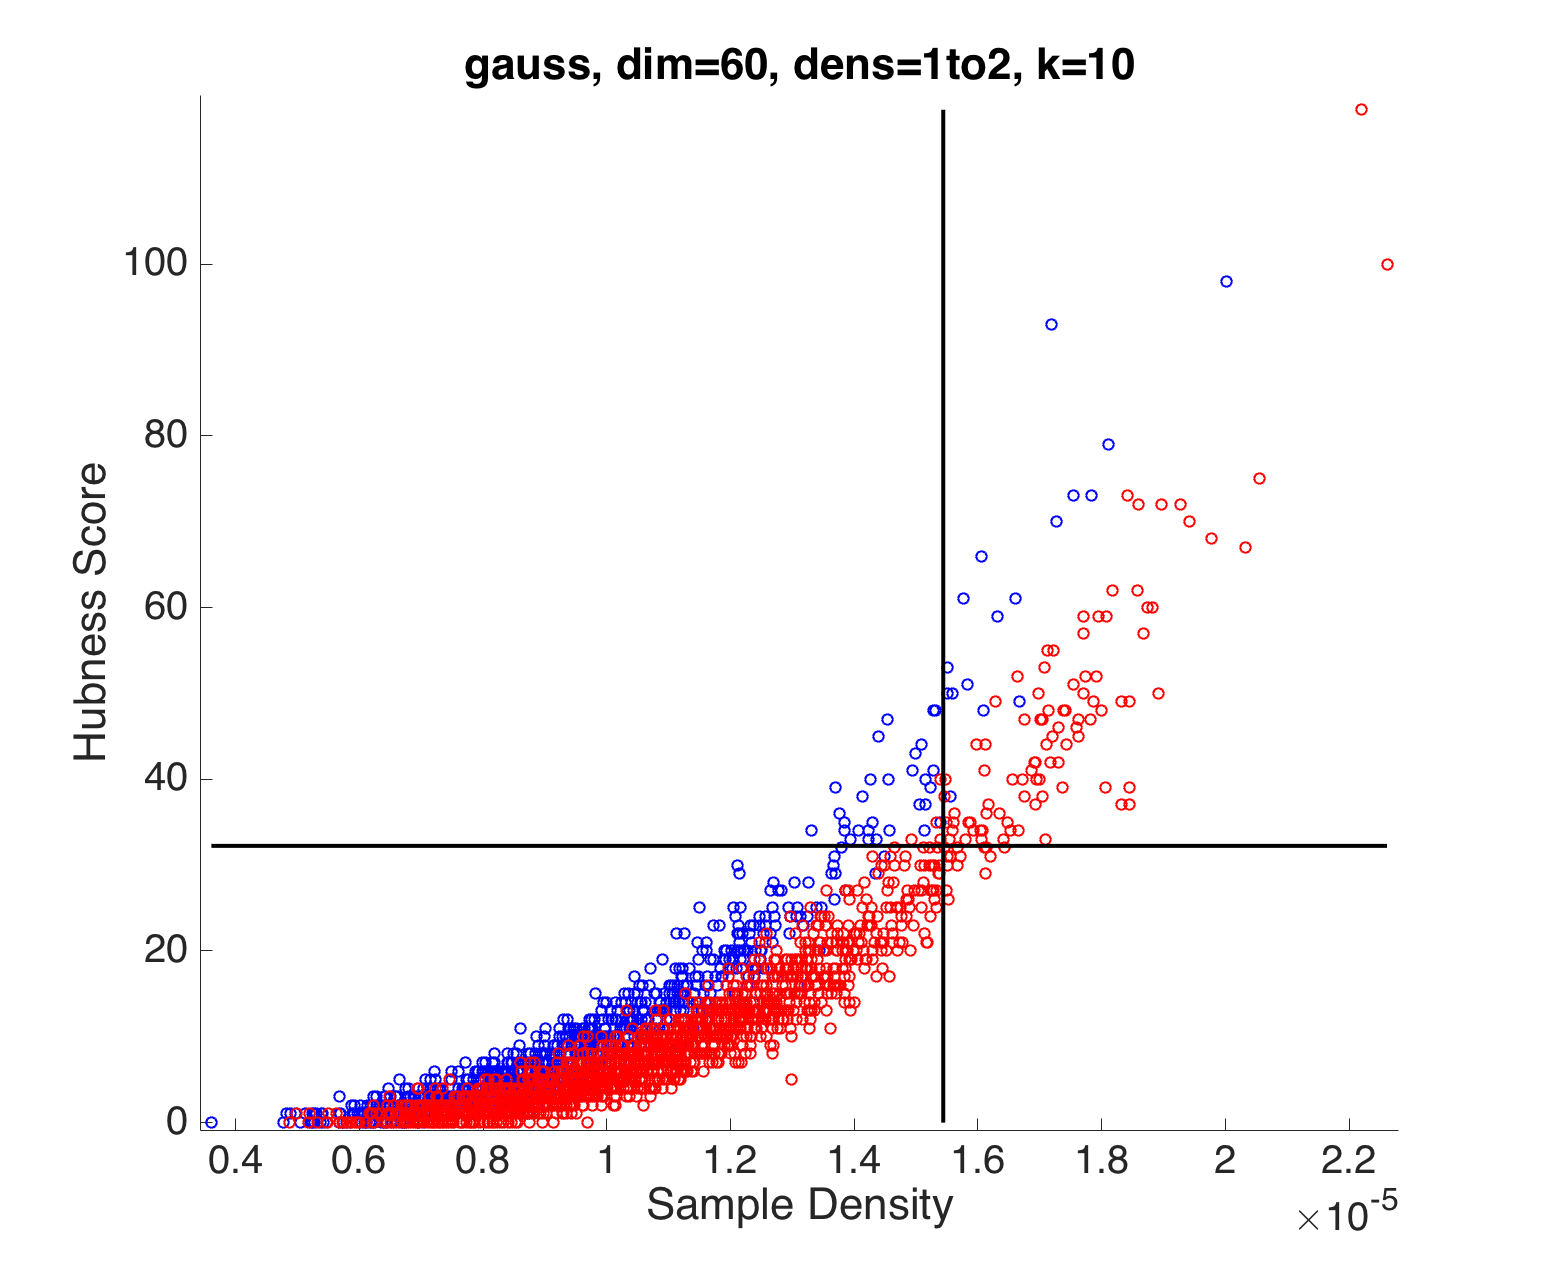
\includegraphics[width=2.5in,height=2in]{../fig/gauss-dim60-1to2-k10-GlobKDEGlobHubs.png} &
        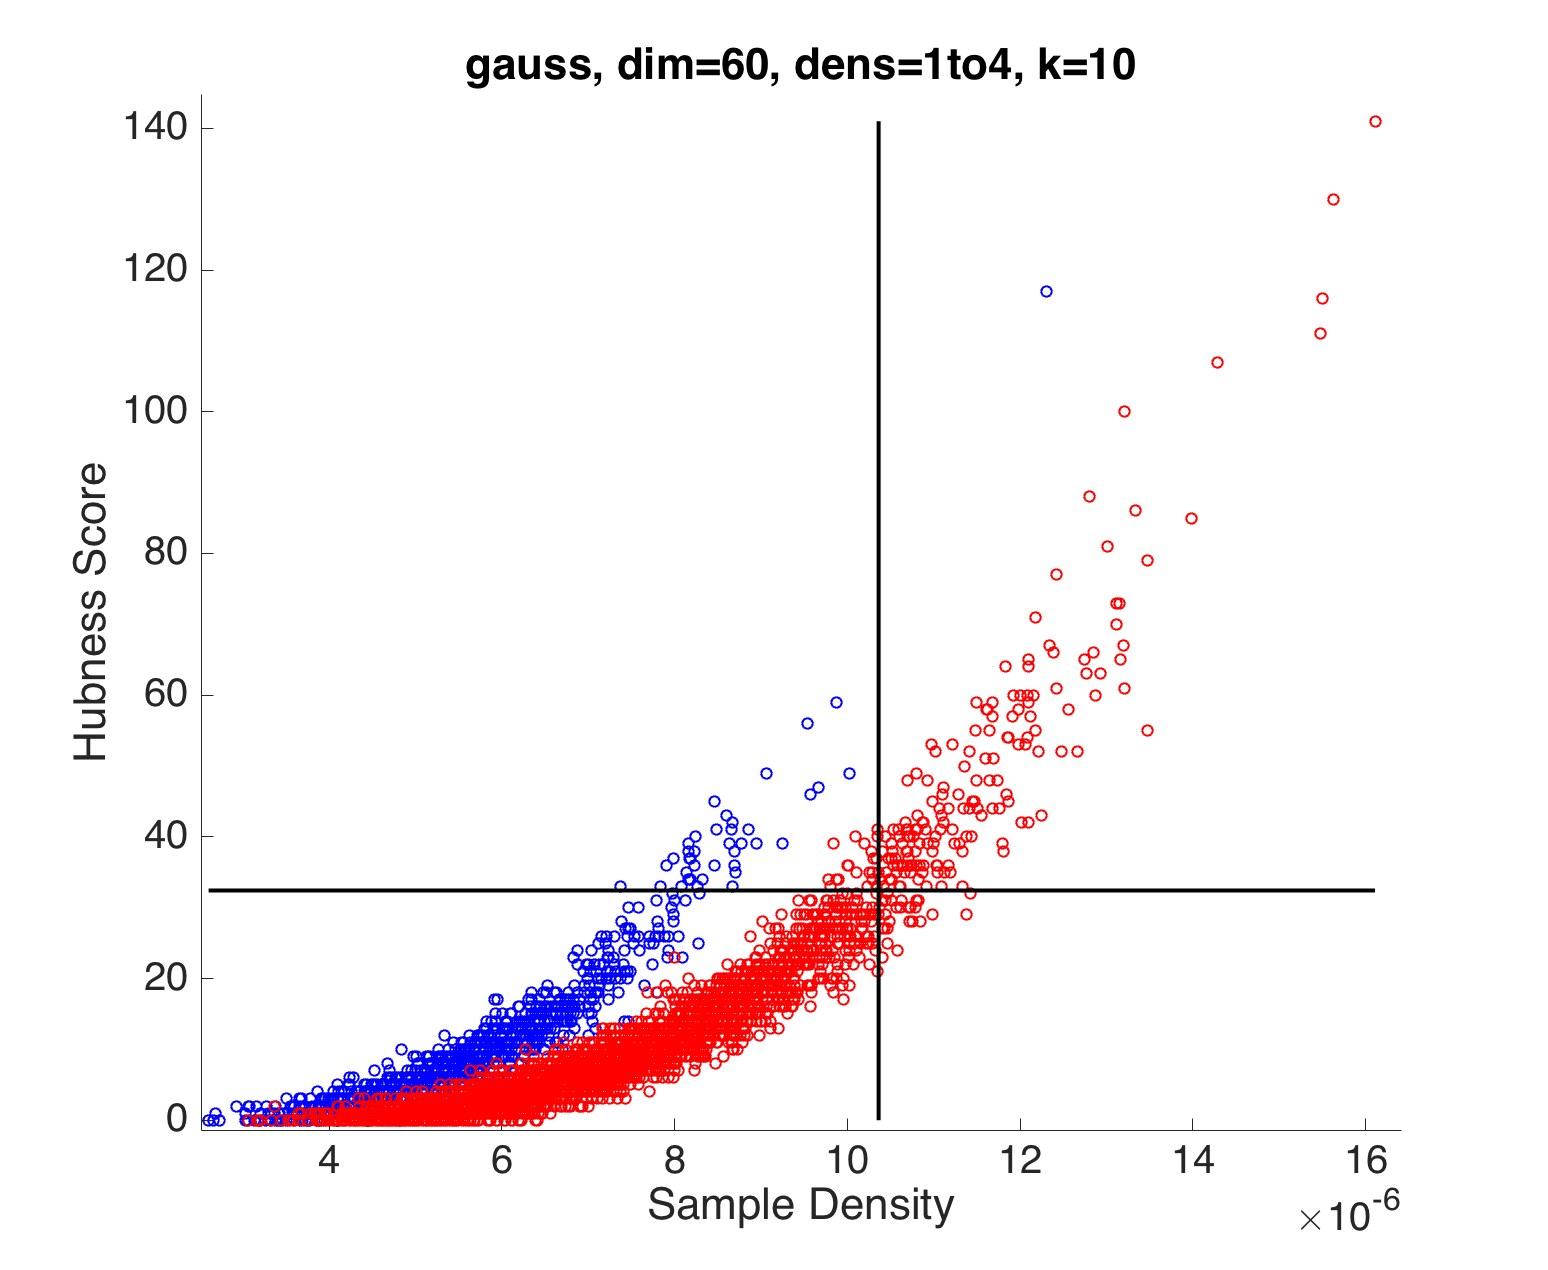
\includegraphics[width=2.5in,height=2in]{../fig/gauss-dim60-1to4-k10-GlobKDEGlobHubs.png} \\
        {\scriptsize (a)} &  {\scriptsize (b)} \\
        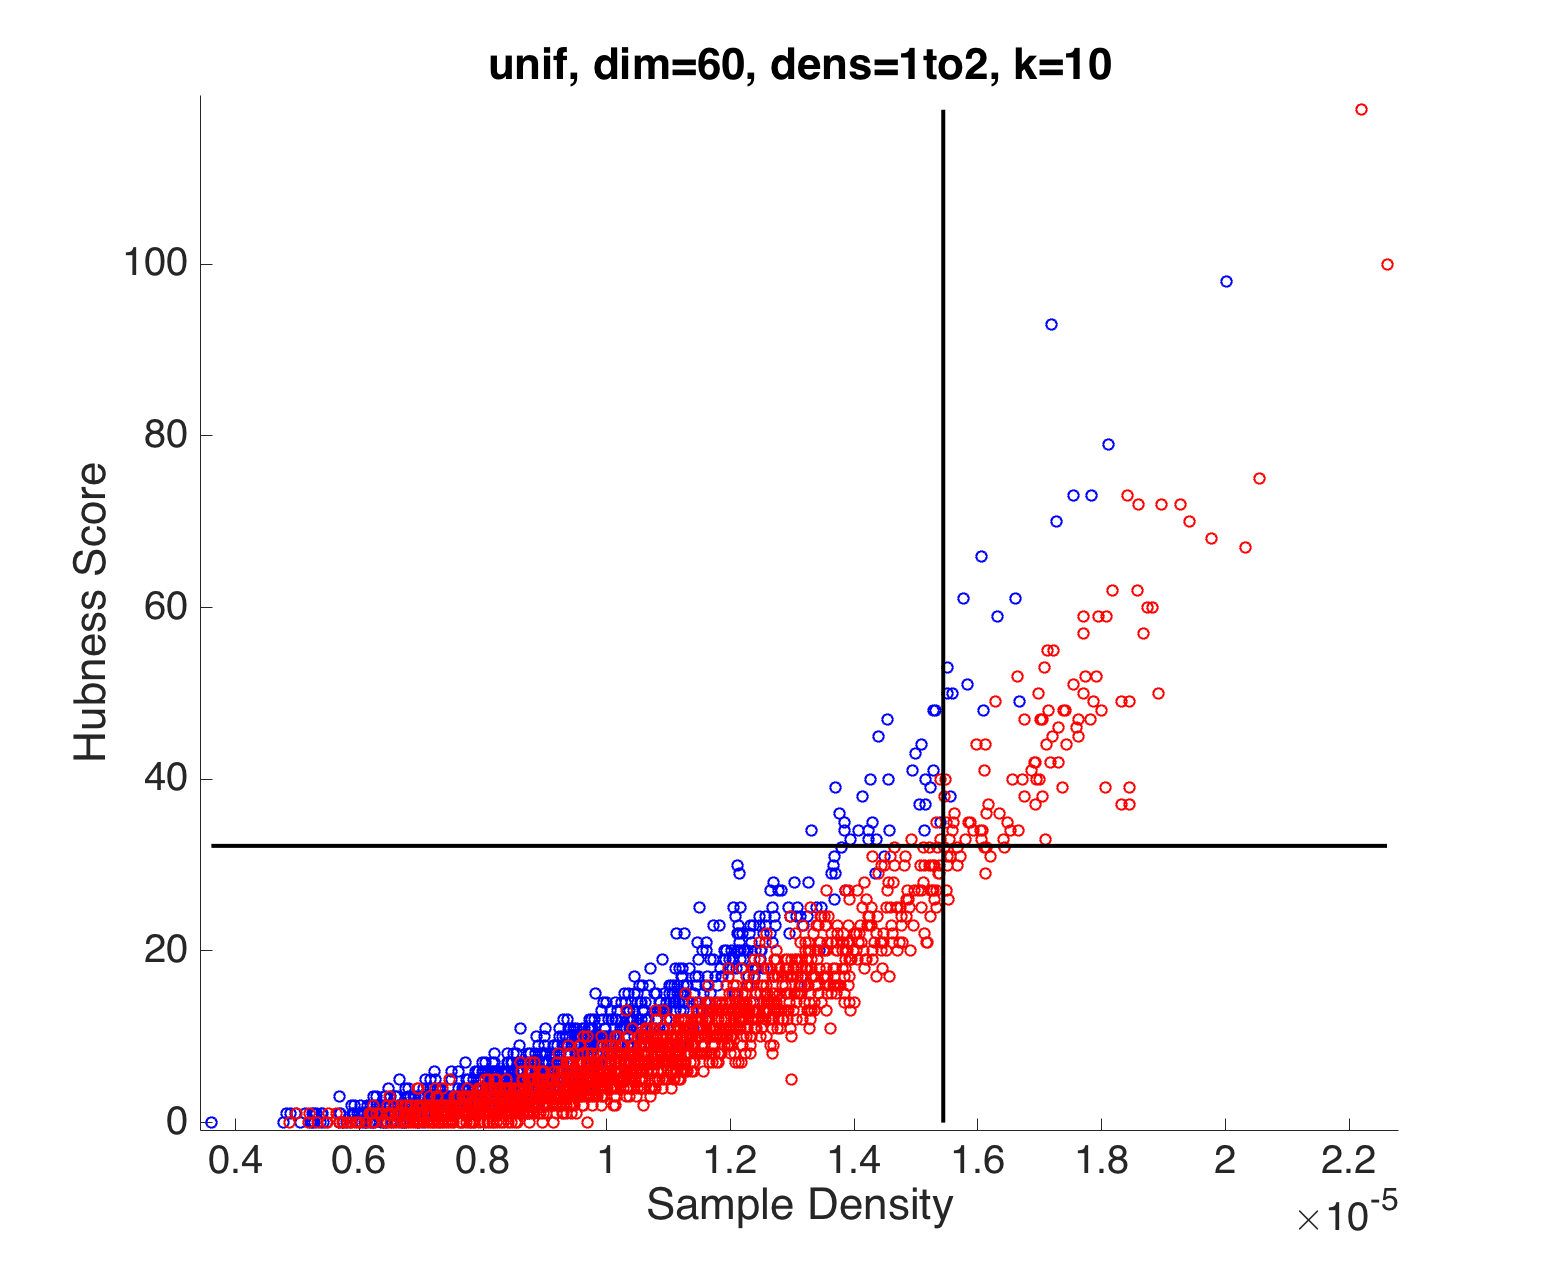
\includegraphics[width=2.5in,height=2in]{../fig/unif-dim60-1to2-k10-GlobKDEGlobHubs.png}&
        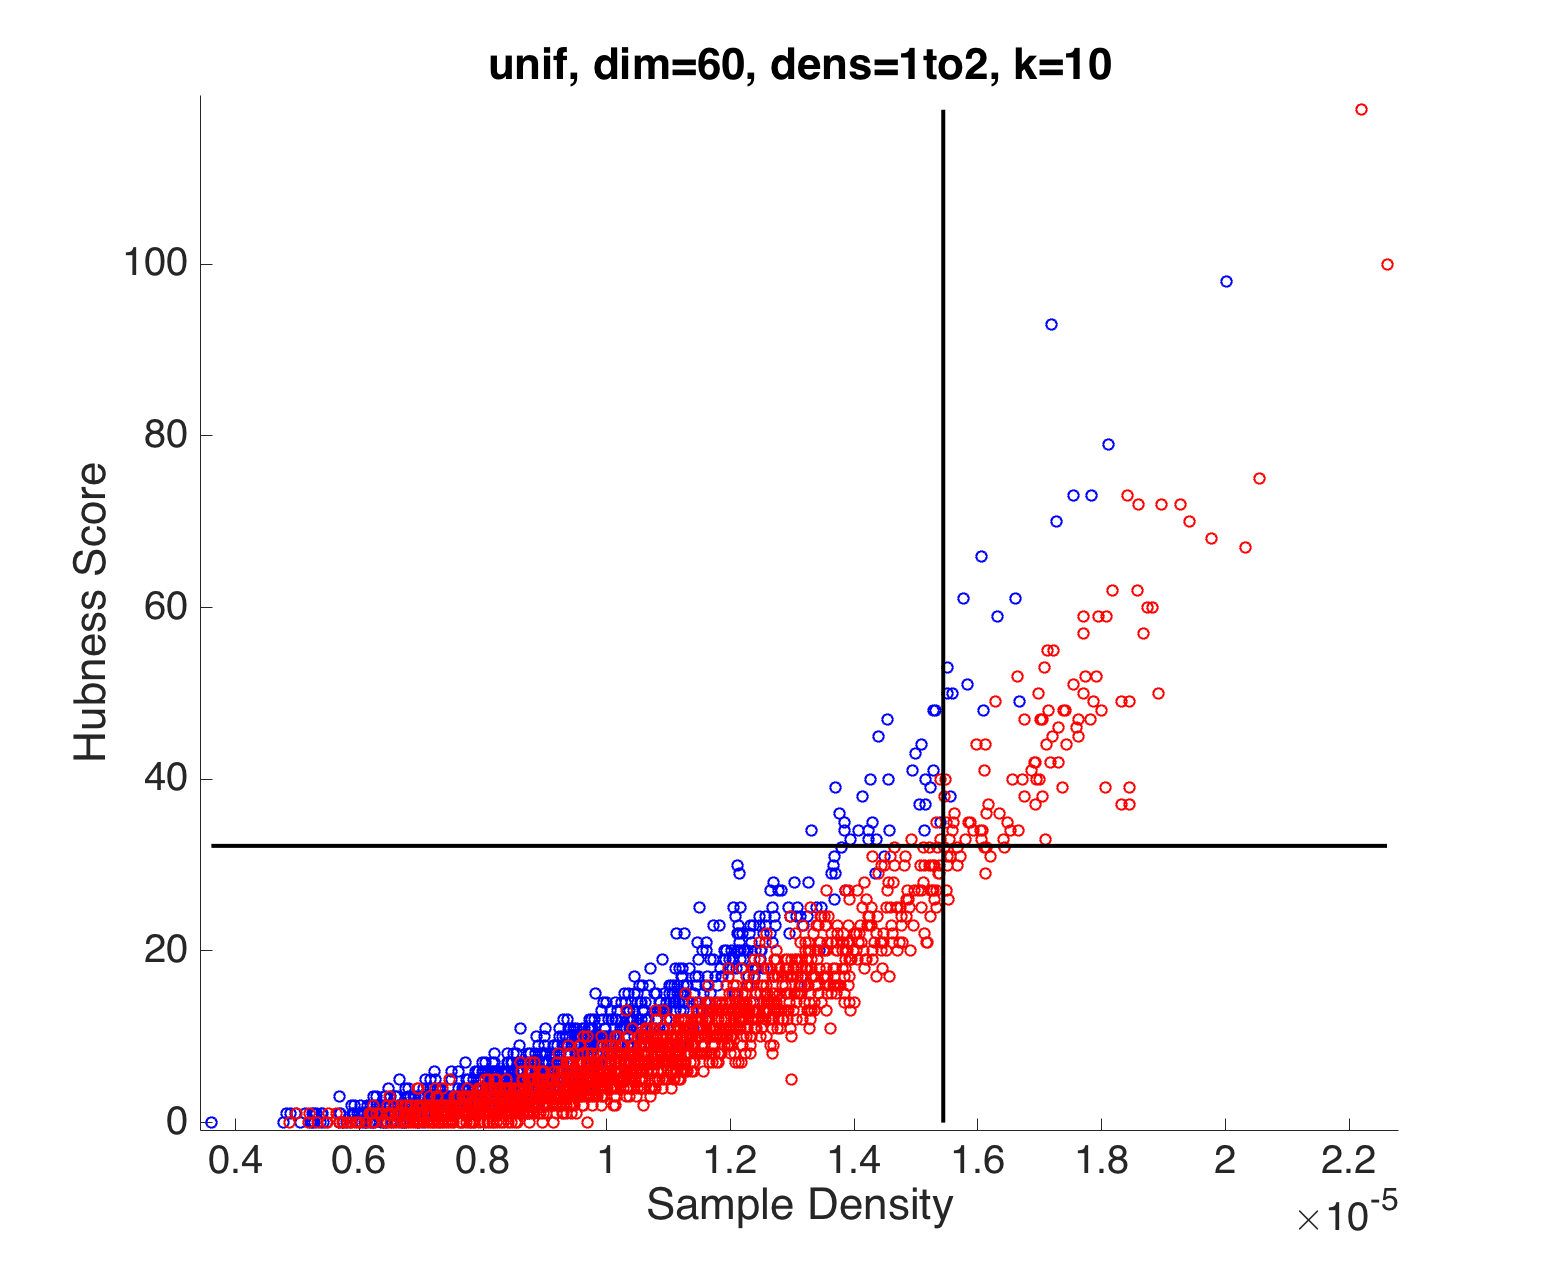
\includegraphics[width=2.5in,height=2in]{../fig/unif-dim60-1to2-k10-GlobKDEGlobHubs.png}\\
        {\scriptsize (c)} &  {\scriptsize (d)} 
      \end{tabular}
      \caption{KDE, $\hat{q}$, plotted against hubness score, $N_{10}$, for data sets (a) $G_{60,3000}$, (b) $G_{60,5000}$, (c) $U_{60,3000}$, and (d) $U_{60,5000}$. The true class is depicted in the two colors of the points and the global thresholds are plotted in black.}\label{fig:GlobDensHubs}
\end{figure}

While in these results points actually appeared in all four quadrants, there is a strong positive correlation, shown in Figure \ref{GlobDensHubs}. In all 72 experiments, there is an average of 94.91\% of the data that lies in the third quadrant (non-hub and low density), which is due to how we defined the thresholds. The interesting observations come from the proportions of data in the other quadrants. For the uniform data sets, 72.26\% of all the hubs were in the dense region, while for the gaussian data sets, it is 82.34\%. Similarly, 78.82\% and 82.64\% of the ``dense'' points in the gaussian and uniform data sets, respectively, are also hubs. Therefore hubs are most likely in dense regions and dense regions are largely composed of hubs. An interesting fact to note is that another density estimator is one over the distance to the $k$-nearest neighbor, which is related to the hubness score. This fact and the evidence from our experiments, we hypothesize that hubness will be closely related to density and in the future will be trying to mathematically express and prove this relationship.

The same experiments were performed but this time with ``local thresholds'', meaning that the same $N_k$ and $\hat{q}$ were used, but this time the mean and standard deviation were calculated for each class. The thresholds for the light blue cluster were plotted in dark blue and the ones for the pink one were plotted in red. Some of the resulting plots can be seen in Fig \ref{fig:LocDensHubs}. For these experiments, the same but stronger pattern was observed. Taking into account all the experiments, an average of 85\% of the hubs were in the high density region, and 84.74\% of the points in the high density region were hubs. The standard deviation for both of these averages was about 0.07. This again supports that hubness scores and density are closely related. 

\begin{figure}
\centering
    \begin{tabular}{cccc}
        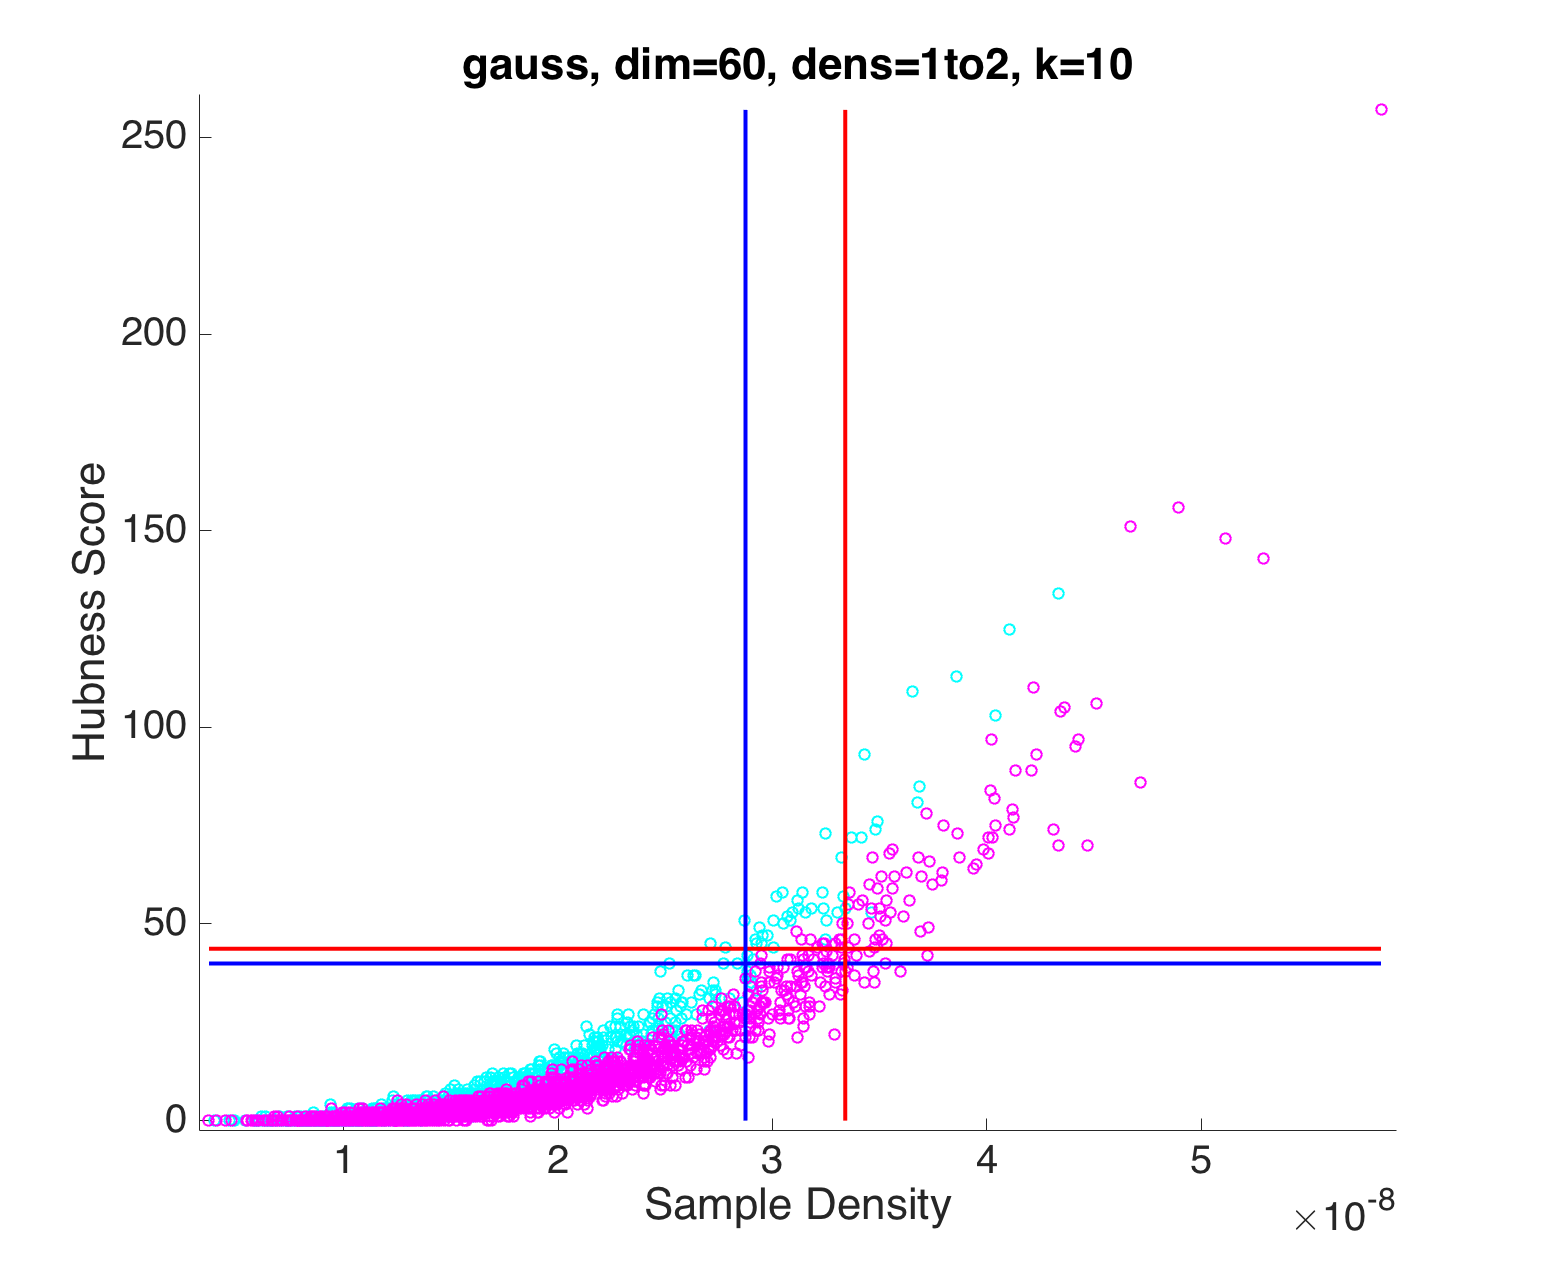
\includegraphics[width=2.5in,height=2in]{../fig/gauss-dim60-1to2-k10-LocKDELocHubs.png} &
        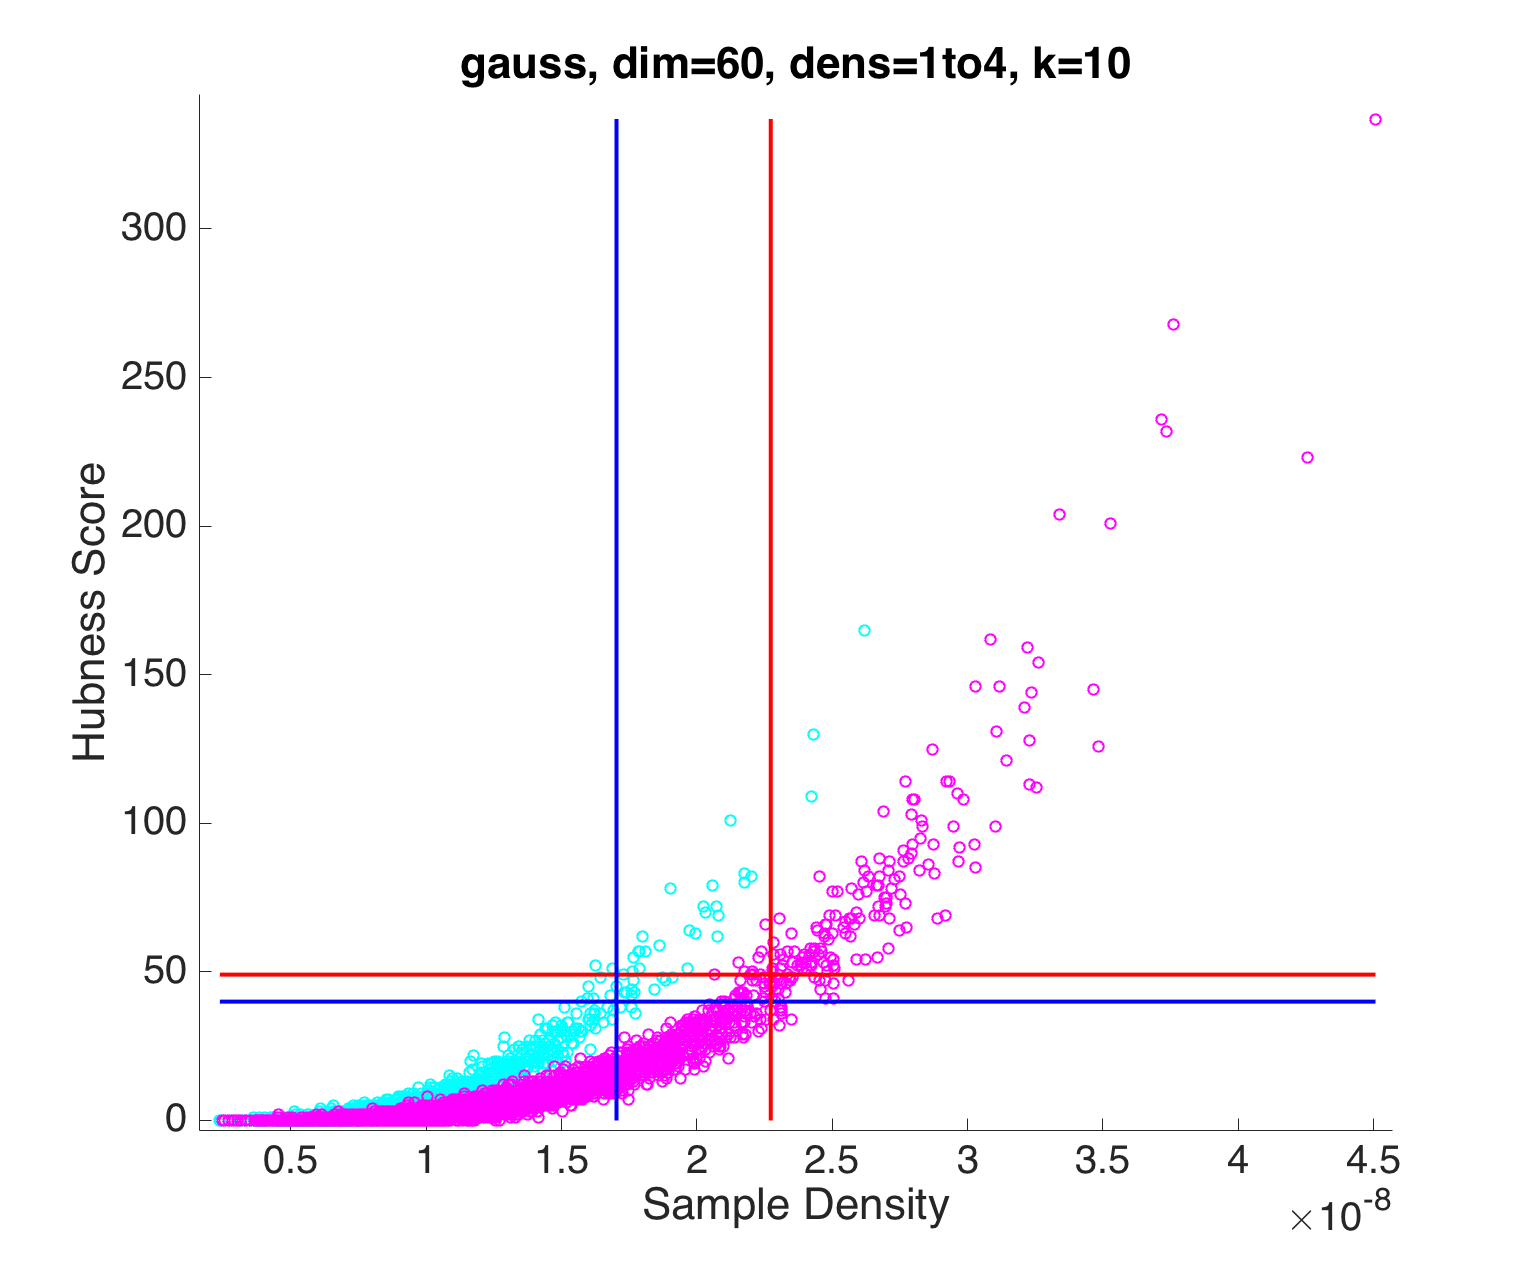
\includegraphics[width=2.5in,height=2in]{../fig/gauss-dim60-1to4-k10-LocKDELocHubs.png} \\
        {\scriptsize (a)} &  {\scriptsize (b)} \\
        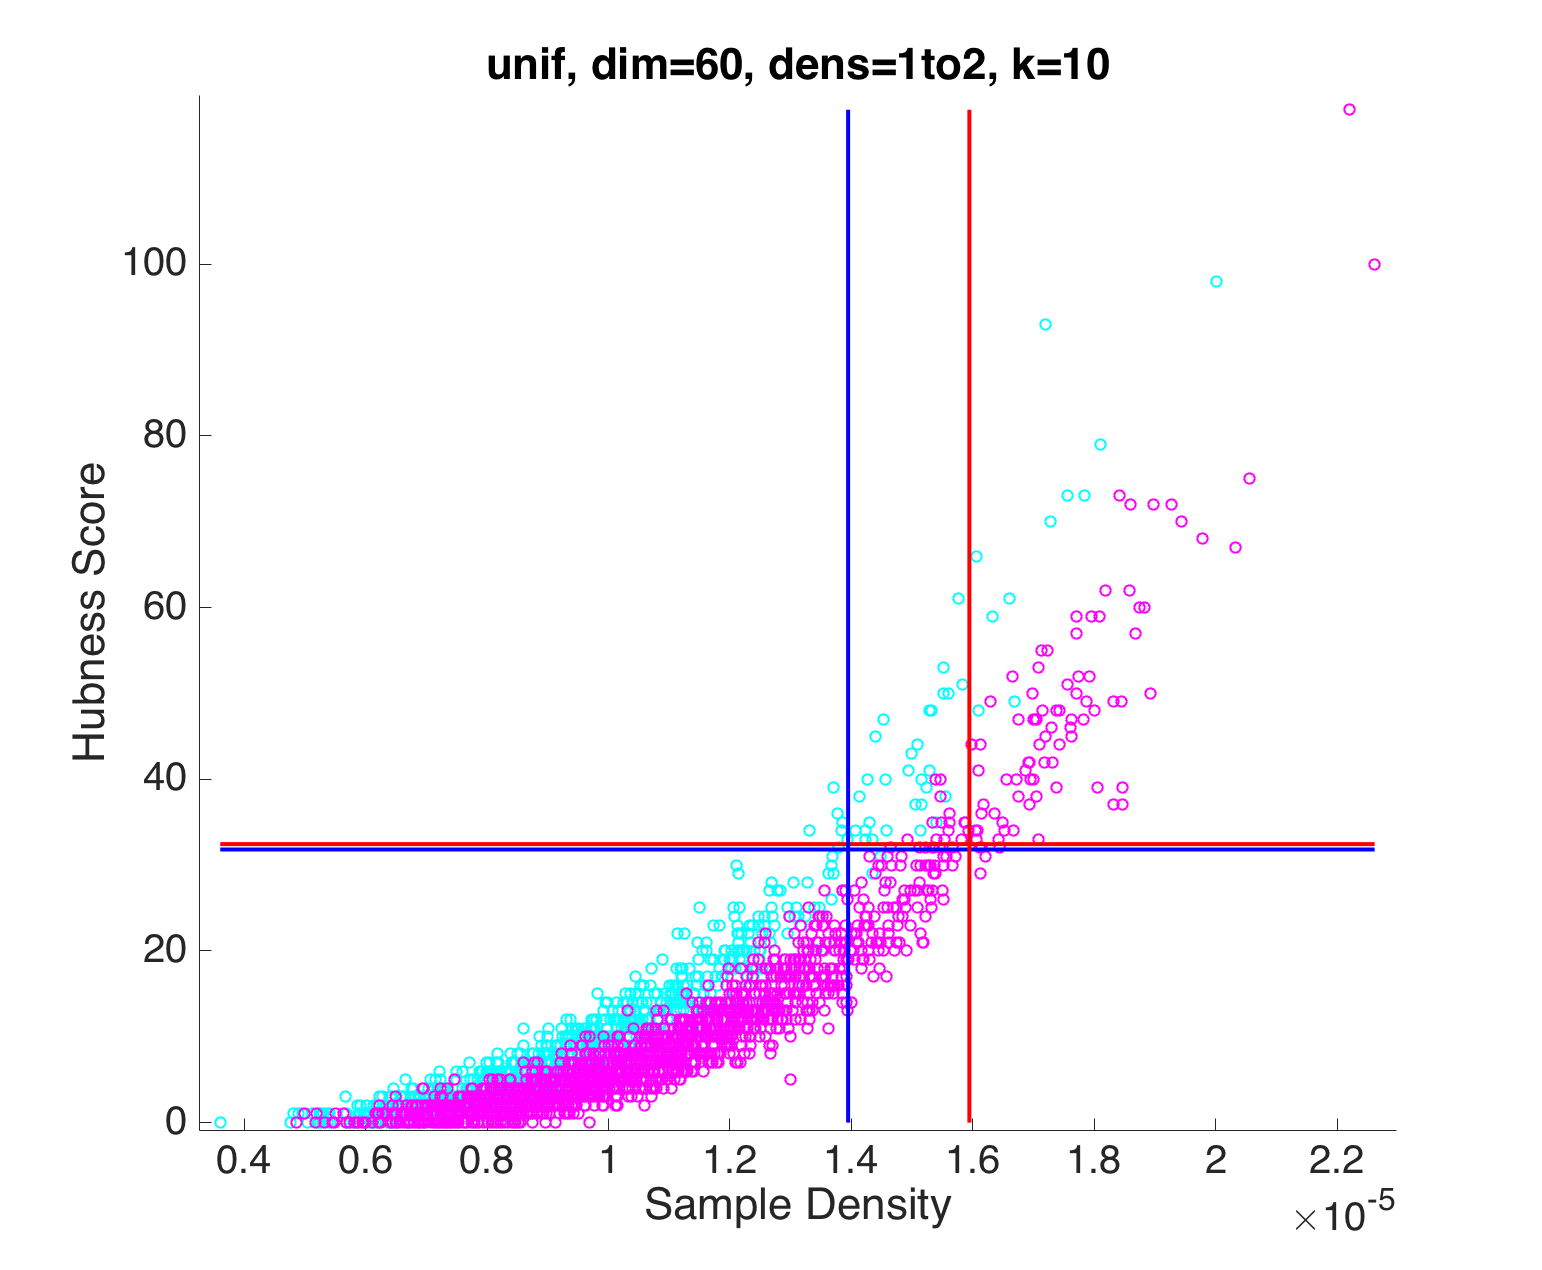
\includegraphics[width=2.5in,height=2in]{../fig/unif-dim60-1to2-k10-LocKDELocHubs.png}&
        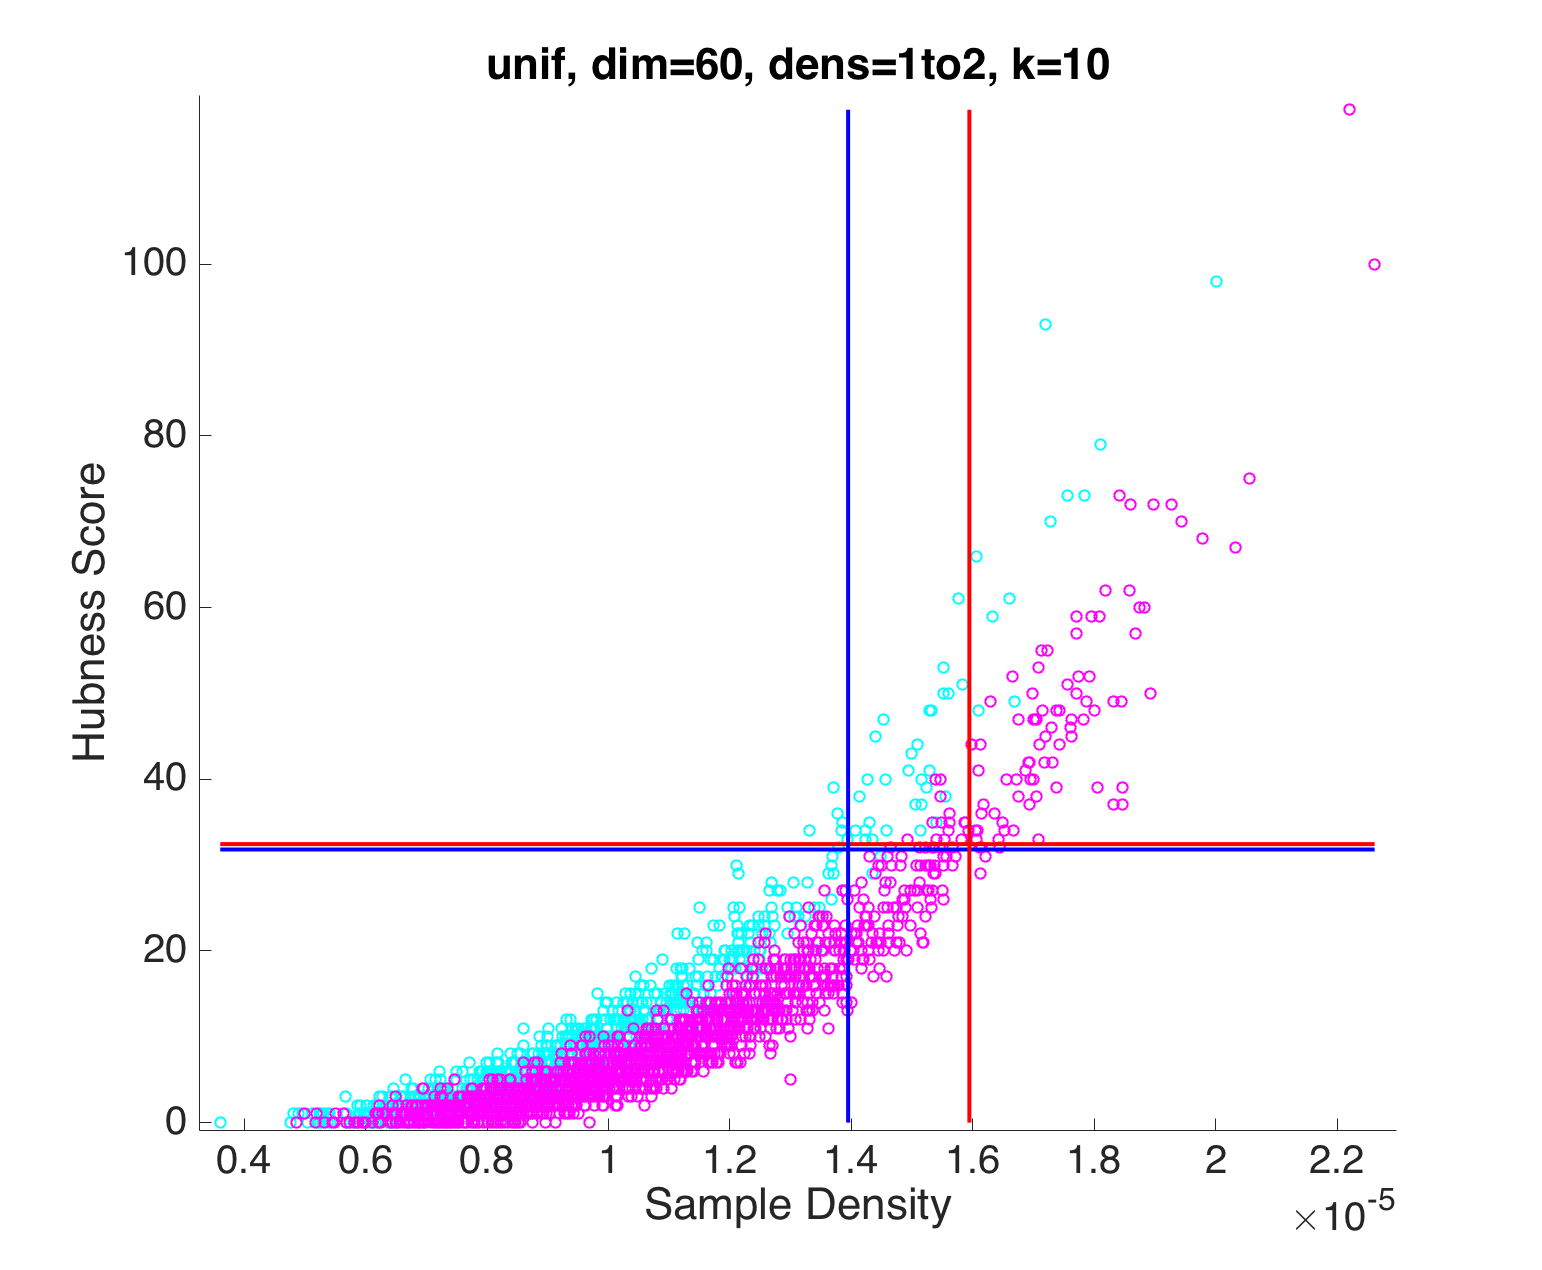
\includegraphics[width=2.5in,height=2in]{../fig/unif-dim60-1to2-k10-LocKDELocHubs.png}\\
        {\scriptsize (c)} &  {\scriptsize (d)} 
      \end{tabular}
      \caption{KDE, $\hat{q}$, plotted against hubness score, $N_{10}$, for data sets (a) $G_{60,3000}$, (b) $G_{60,5000}$, (c) $U_{60,3000}$, and (d) $U_{60,5000}$. The true class is depicted in the two colors: pink and blue. Class thresholds are plotted in red (for the pink class) and blue (for the blue class).}\label{fig:LocDensHubs}
\end{figure}
 
While the local thresholds are informative since it removes the effects of the difference in densities, in the real world one can only see the global thresholds. Since hubs are being used to do clustering procedures, it is reassuring to see how even though high density regions can lack points from the smaller cluster, hubs appear from both clusters. Also, there is not a big difference between the ``local'' and ``global'' thresholds, so this gives a sense of ``robustness'' to density that needs to be further explored and exploited.

Another interesting observation from all the experiments, both the local and global thresholds, are the ``wings'' formed by the two clusters. The experiments show that the bigger the difference in densities between the two clusters, the more of a gap there is, and hence forming the ``wings.'' Due to the curse of dimensionality, these wings are more common in the 30 and 60 dimensional data than they are in the 100 dimensional data. However, it would be interesting to further explore what gives rise to the ``wings'' and under what other conditions these are seen.

[Distance plots, Correlation of hubs to density, etc.]

\subsection{Hubness and Purity}
\label{purityHubness}

Hubs have the potential to be used in a clustering method. For example, it is possible to only cluster hubs and then assign their corresponding reverse k-nearest neighbors(RkNN), or those points that have hubs as their k-nearest neighbors, the same labeling as the hubs. Hence, we explored the relationship between hubness score and purity, which is defined as:

\[
\mbox{purity } = \frac{1}{N} \sum_i \max_j |\hat{C}_i \cap C_j|
\]

where $\mathcal{C} = \{\hat{C}_1,\cdots,\hat{C}_p\}$ is the set of calculated clusters and $\mathbb{C} = \{C_1,\cdots C_q\}$ is the set of true classes in the data.

To explore that relationship, all the points in the data set such that $N_k > \lambda$ were chosen and their corresponding true labels, which are treated as $\mathcal{C}$ to avoid calculation errors in this exploratory step, were recorded. For each point that passed the hubness score threshold, their RkNN were assigned the same cluster label. Once that is done for all points that passed the threshold, purity was calculated.

The plots for these experiments show the purity levels given threshold values of $N_k$ and the black vertical line show 2 standard deviations away from the mean of $N_k$. We expected a monotonic increasing function, meaning that the larger the hubness score the better purity we expected, and higher purity results for the convex clusters. For the Gaussian and Uniform data sets, purity was 1 for all the experiments. This is not very surprising since in the convex and well separated cases, the k-nearest neighbors are going to be other points in the same cluster. Therefore, if you know the true labels for those points, then the clustering will lead to high accuracy, or in this case high purity. There was a more interesting behavior for the non-convex data, shown in Figure \ref{fig:purity}(a). While in all these experiments, purity eventually does achieve a value of 1, it happens at 10,12, and 11 standard deviations above the mean for $N_{5}, N_{10},$ and $N_{50}$, respectively. These are much higher values than the current hub cut off, which is 2 standard deviations from the mean. Most importantly, purity values reach 1 when all the points from one cluster are gone. Therefore, the important region is the one before this leveling off, which has purity peaks of 0.8888, 0.88, 0.85, respectively.

\begin{figure}
\centering
    \begin{tabular}{cccc}
        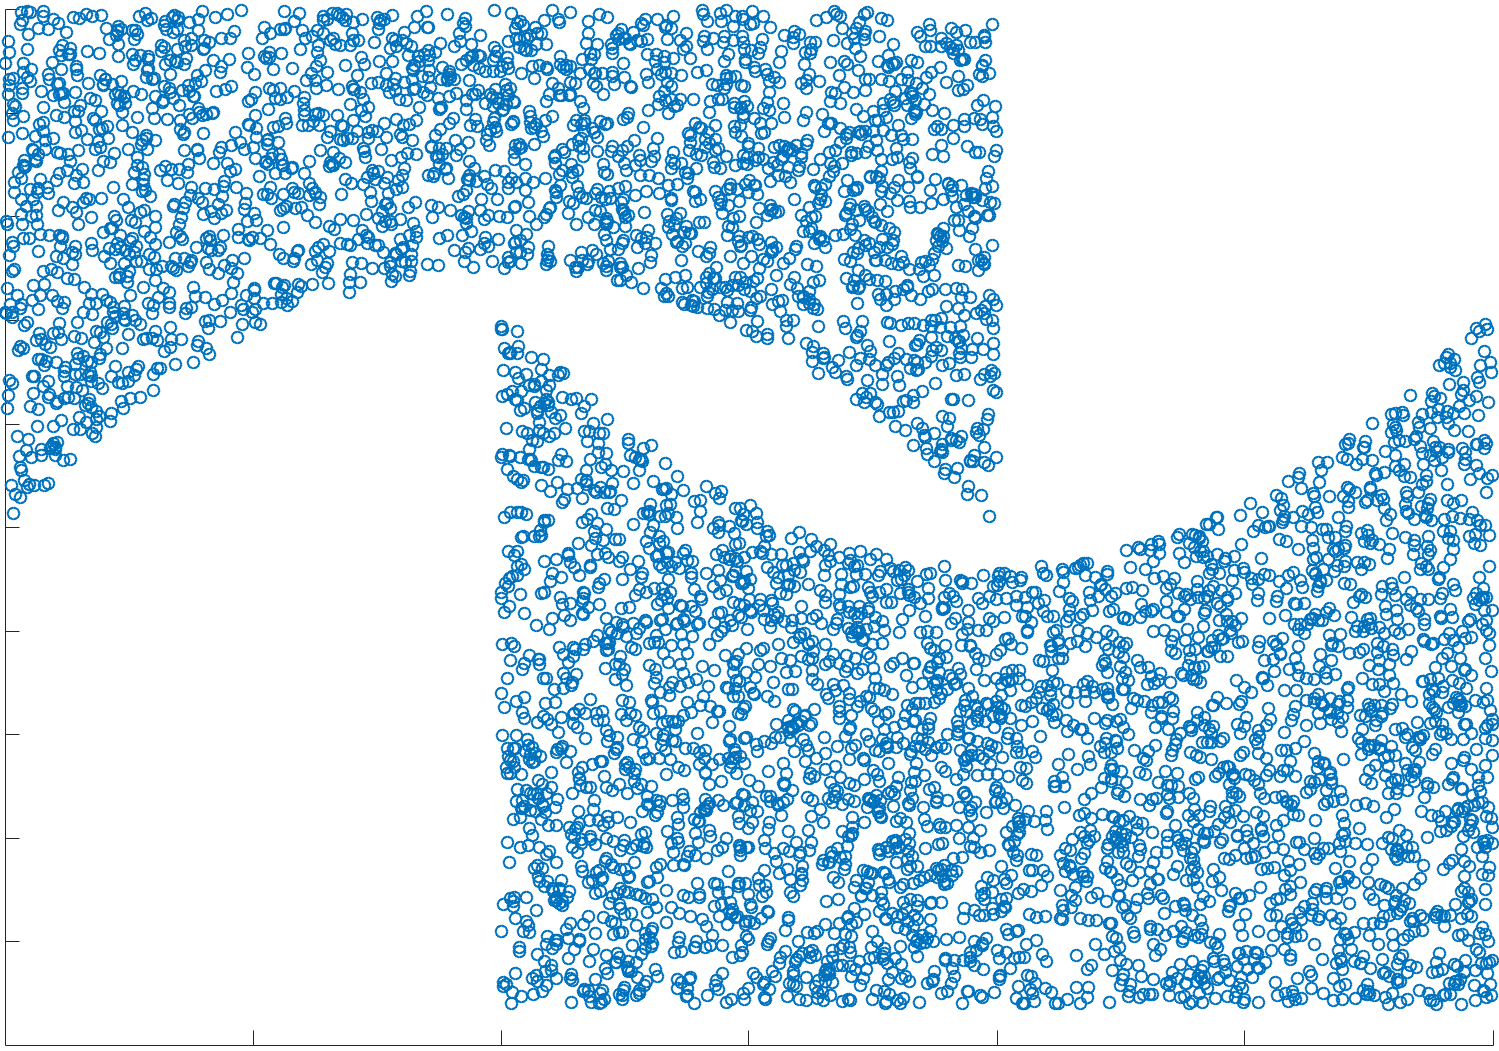
\includegraphics[width=2.5in,height=2in]{../fig/SQdata.png} &
        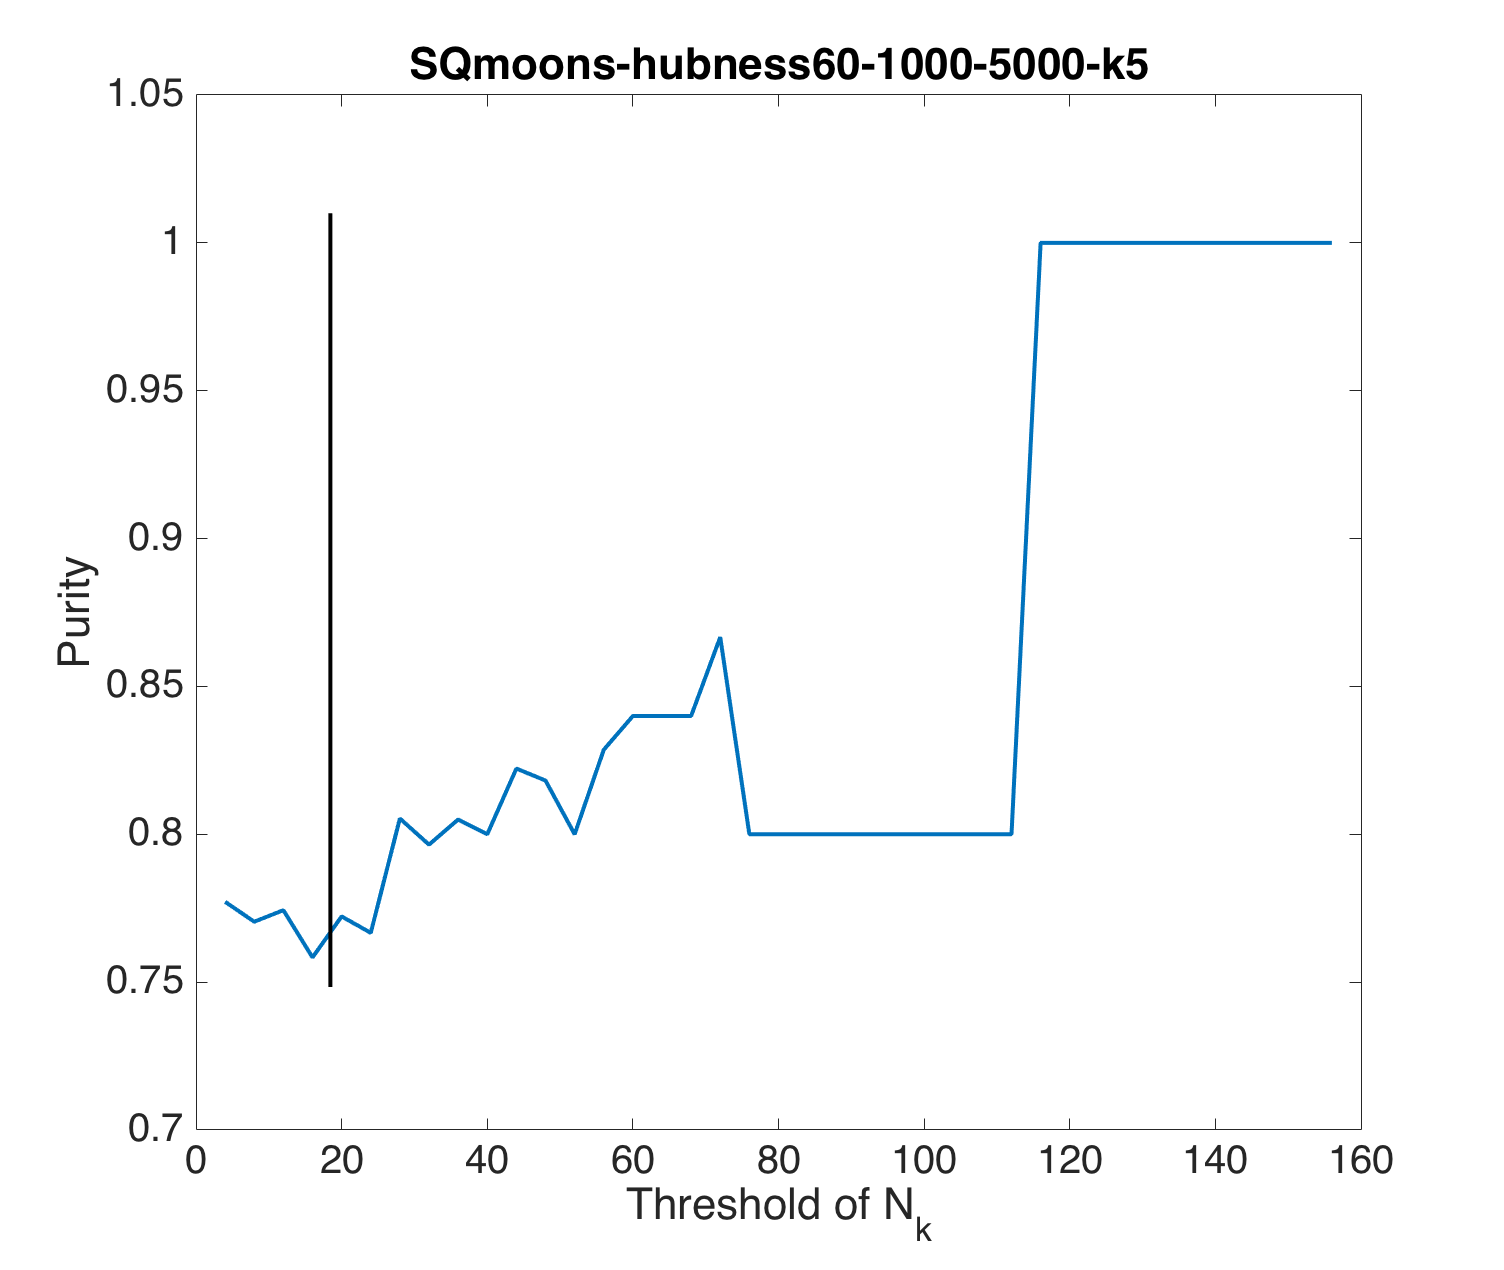
\includegraphics[width=2.5in,height=2in]{../fig/SQmoons-dim60-6000-k5-PurityHubness.png} \\
        {\scriptsize (a)} &  {\scriptsize (b)} \\
        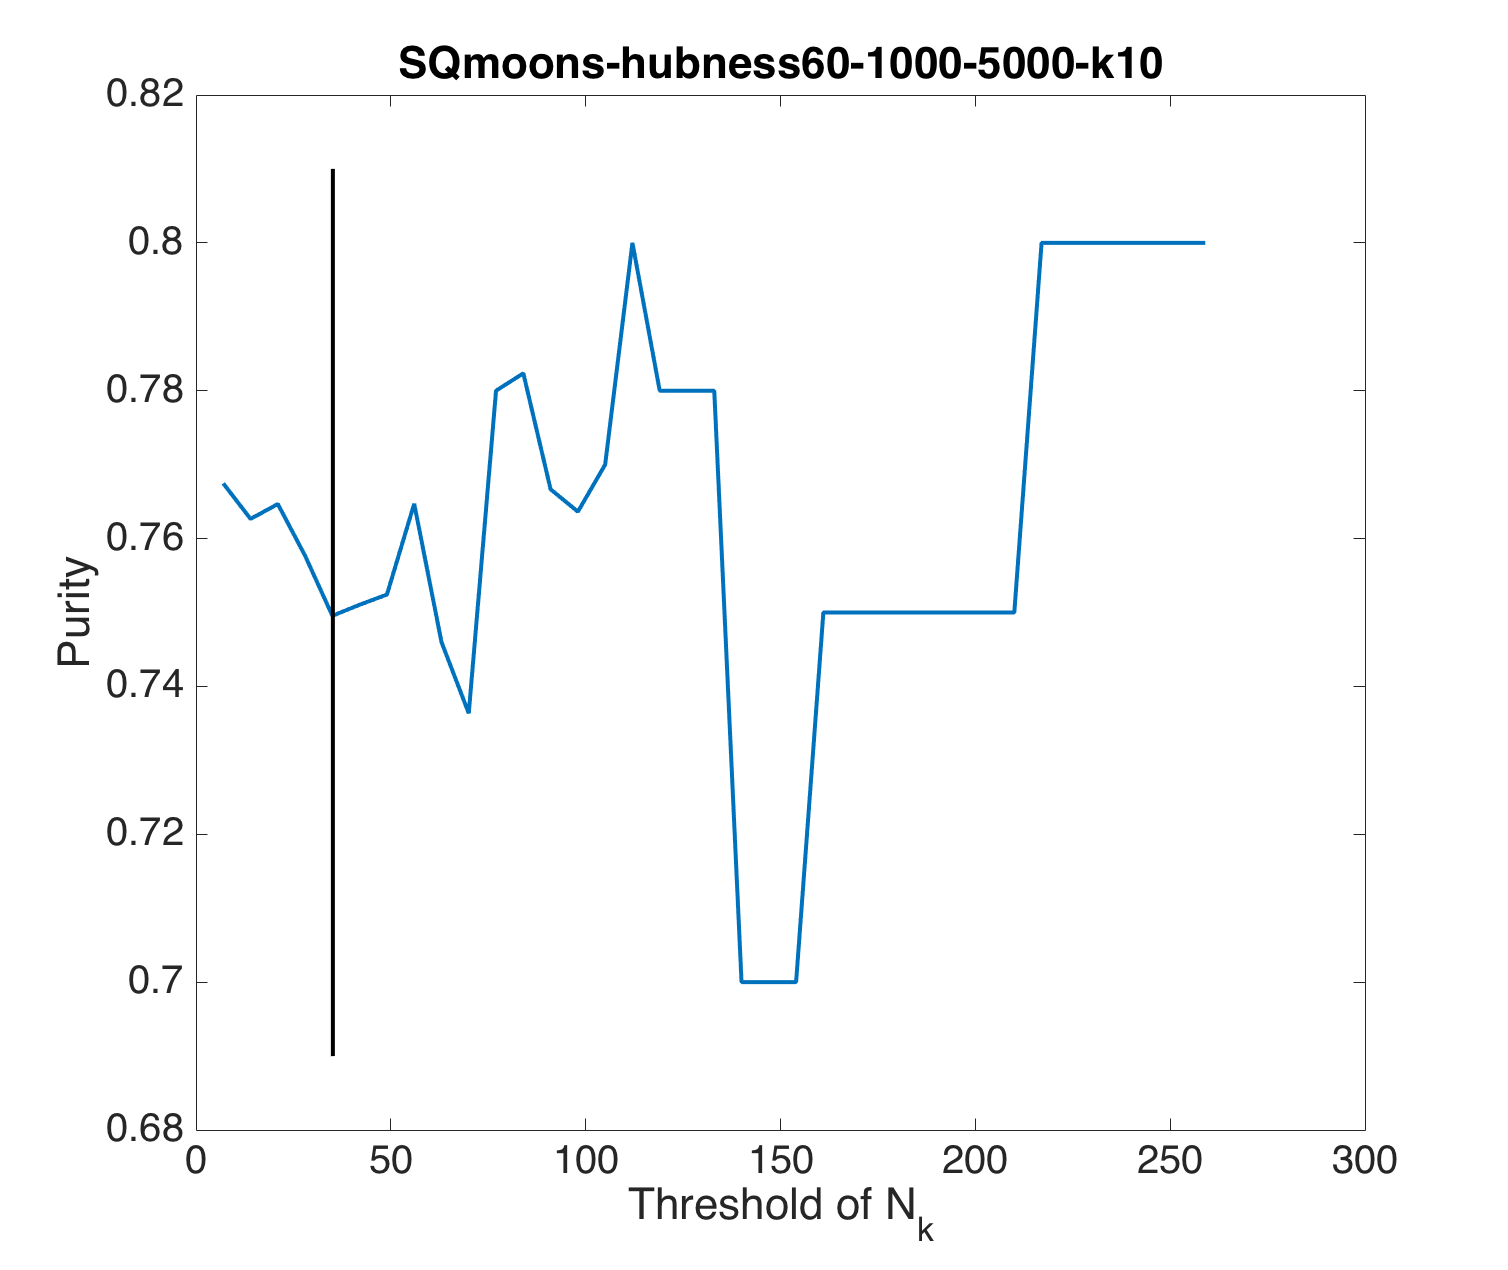
\includegraphics[width=2.5in,height=2in]{../fig/SQmoons-dim60-6000-k10-PurityHubness.png}&
        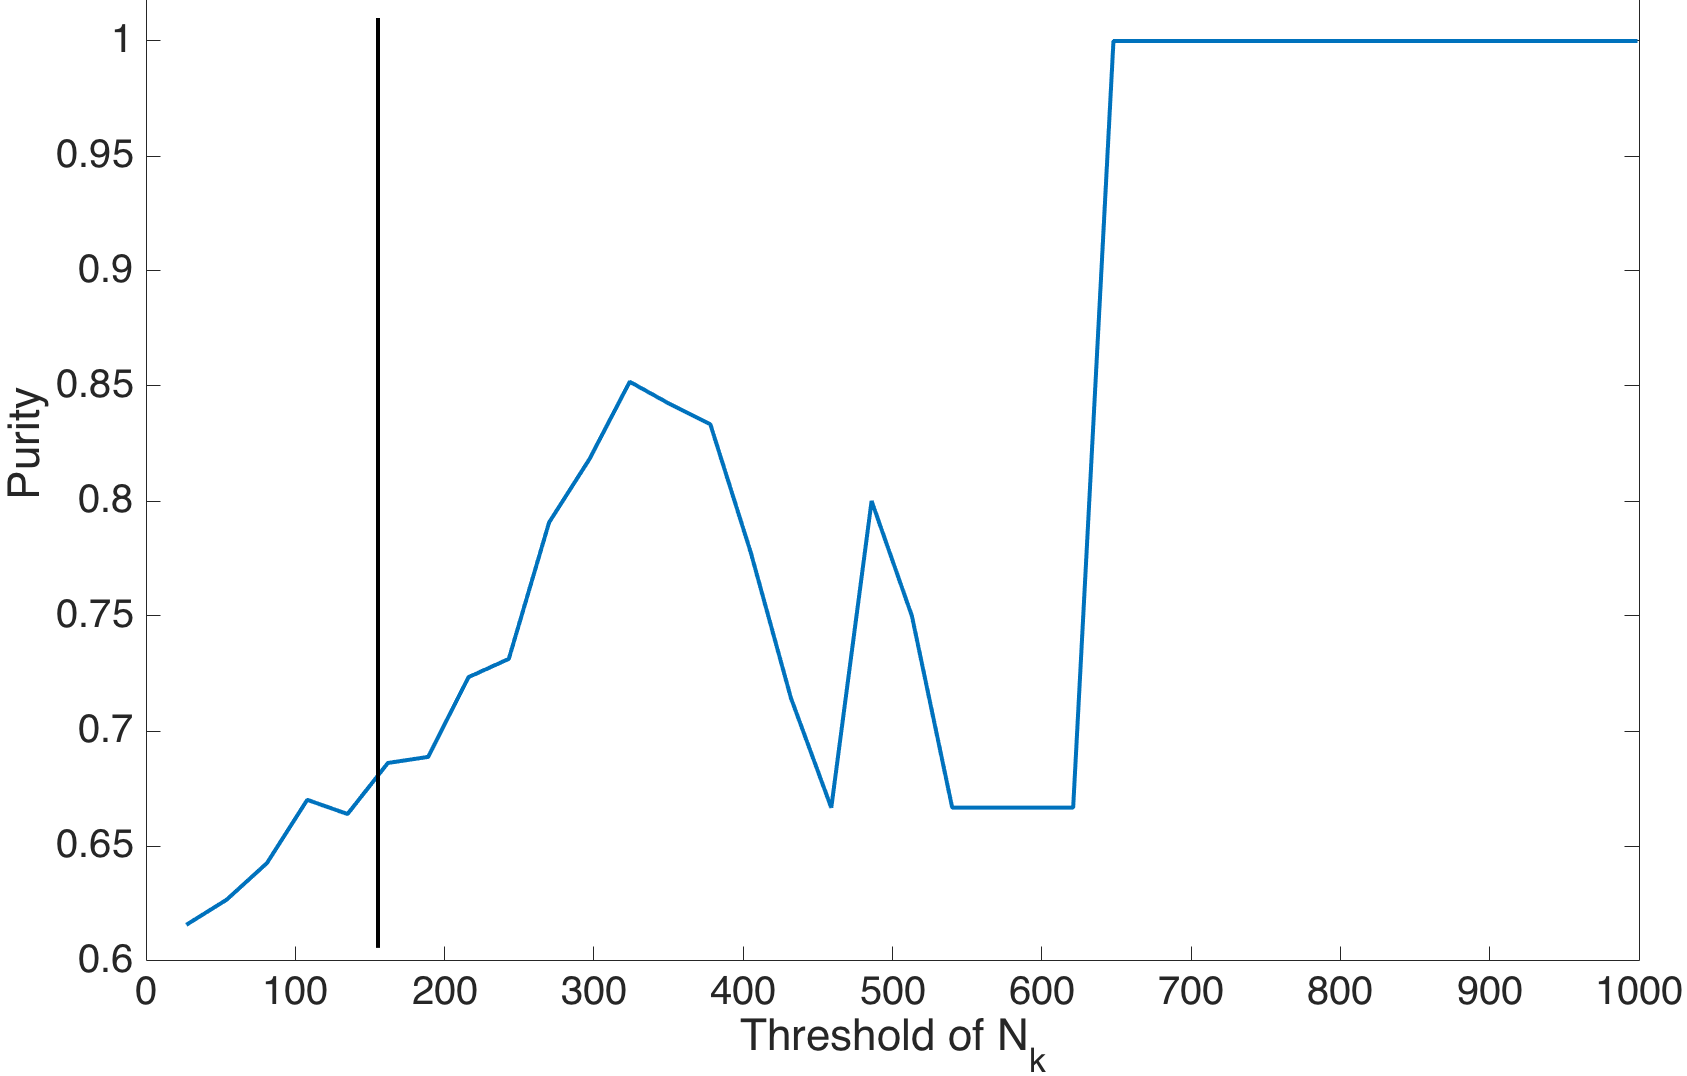
\includegraphics[width=2.5in,height=2in]{../fig/SQmoons-dim60-6000-k50-PurityHubness.png}\\
        {\scriptsize (c)} &  {\scriptsize (d)} 
      \end{tabular}
      \caption{(a) The first 2 coordinates of the non-convex data set. The hubness score with $k$ = (a)5, (b)10, (c)50 plotted against purity. The black vertical line shows 2 standard deviations above the mean of the hubness score so that all the values to the right will be considered hubs. }\label{fig:purity}
\end{figure}



\section{Discussion}
\label{sec:5}



\section{Conclusion and Future Work}
\label{sec:6}

%\input{referenc}
\end{document}